\part{Introduction}

    \chapter{Overview}

        This project is focused on integrating new technological developments, like smartphones and wearable devices, into medical data acquisition so that healthcare professionals have the capability to make use of large amounts of data related to physical activity and physiology to inform their decision-making when managing the health of individuals. Up until now, in order to capture data from a patient, the patient would have to visit their General Practitioner (GP) or a healthcare professional had to visit the patient; this is costly in both time and financial resources, so this project seeks to lessen some of these barriers. 

        By using sensors provided in smartphones and wearables, this project seeks to monitor and quantify daily activities that are strongly related to a patient's health, like walking and sleeping.

    \chapter{Motivation}

        \section{Pulmonary Disease and Heart Failure}

            Chronic diseases are defined as health problems that require on-going management and treatment for years or decades \cite{chronic_diseases}. In the UK, 17.5 million people have a chronic disease, two-thirds of these are aged 75 or older. This presents a large financial and logistic challenge as these patients with these conditions require long term care. In the US, chronic diseases affect 130 million people, which generates around \$1.4 trillion a year in healthcare costs \cite{chronic_diseases} or \$10.77 per patient per year. Two of these diseases are Chornic Obstructive Pulmonary Disease (COPD) and heart failure. 

            Chronic Obstructive Pulmonary Disease and heart failure affects a person's ability to engage in physical activity and both tend affect a similar group of people \cite{copd_nhs, heart_failure_stats}. By monitoring a person, who is suffering from either of these diseases, for example their activity levels and quantity or quality of sleep, a healthcare professional may be able to track the person's condition and prevent a costly hospital admission.

            Chronic Obstructive Pulmonary Disease (COPD) is the name for a set of lung conditions that are the source of breathing difficulties. COPD is a relatively common disease for middle-aged or older adults. According to the British Lung Foundation, around 4.5\% of adults aged 45 or above are diagnosed with this condition \cite{copd_stats}. Often, the person affected does not realize that they have the disease, but their breathing problems get gradually worse. The disease cannot be cured or reversed, but treatment may keep it under control so that it does not impact on daily life. Part of this treatment may be what is known as 'pulmonary rehabilitation', a specialised programme of exercise. \cite{copd_nhs}.

            Heart failure is a condition where the heart is unable to pump blood around the body properly, which usually occurs because the heart is too stiff or weak. According to the British Heart Foundation, around half a million people in the UK have been diagnosed with heart failure \cite{heart_failure_stats}. There are four classes or stages of heart failure, with a higher class signifying higher severity. 

        \section{Six Minute Walk Test}

            As mentioned above, COPD and heart failure impact a patient's ability to engage in physical activity. These diseases have no cure and generally tend to get worse with time. In many cases, the degree of physical activity that the patient can undergo indicates the severity of the disease \cite{six_minute_walk_test}. This fact is utilized in the application of the Six Minute Walk Test (6MWT).

            The Six Minute Walk Test (6MWT) is a standardized test of functional exercise that involves walking along a flat, straight course for six minutes. The test is self paced and there are no requirements regarding breaks. The 6MWT is often used to track therapy progress and has been proven to be sensitive to common therapies \cite{six_minute_walk_test}. Typically the variable that is measured is the distance walked in the six minutes. However, oxygen saturation and heart rate can be measured too if the proper devices are used during the test.

        \section{Smartphones and Wearables}

            In recent years the penetration of the smartphone has been rapid and widespread. According to the Deloitte Mobile Consumer Survey 2016 \cite{deloitte}, 91\% of people in the UK aged 18-44 own a smartphone. Additionally, Statista reports that in 2015, 50\% of those surveyed aged 55-64 owned a smartphone and 18\% aged 65+ owned a smartphone \cite{statista}. Clearly, the adoption of the smartphone is reaching saturation among the general population below 45.

            Parallel to the increasing adoption of smartphones are the increasing capabilities of such devices. For example, the BLU Energy Diamond M Android Smartphone which is available for \textsterling39.99 on AmazonUK has a 1.3 GHz quad-core processor and 512MB RAM \cite{new_phone}. This is comparable to flagship devices from earlier years, for example, the Samsung Galaxy S3 released in May 2012 at a cost of \$599 at launch. This device had a 1.4 GHz quad-core processor and 1GB RAM \cite{samsung}. The cost to performance ratio for such devices has decreased dramatically in recent years.

            Another important factor to consider is the availability of sensors in these devices. Even such low-end devices as the BLU Diamond M has a built-in accelerometer and proximity sensor \cite{new_phone}. Higher-end devices will have additional sensors such as a gyroscope, a barometer, or a magnetometer. The availability of sensors allows for a unique opportunity for widespread, remote data collection. 

            For example, the 6MWT described above can be performed by the patient using a certified application that counts the steps automatically. This is easier and less costly than having the patient attend a testing centre to record these results.

            In addition, wearables have also become widespread in the last few years with big players like Apple introducing the Apple Watch in 2015 and Google debuting Android Wear in 2014. Along with these more general-purpose devices are more niche devices like those developed by FitBit or Jawbone that are aimed at fitness enthusiasts. These new devices are packed with sensors and provide another avenue for day-to-day data collection.

    \chapter{Objectives}

        \section{Step Counter}

            In order to track 6MWT performance, a generalized step counting algorithm must be available. More modern smartphones often incorporate step counters on device, but older or cheaper devices still lack this functionality. Applications like Google Fit aim to perform a similar task, however, the details of their algorithms are unknown. In addition, there are wearable devices such as a Fitbit or Jawbone that incorporate step counters based on processing the accelerometer data. Again, the underlying principles of such devices are not published and retrieving the data is usually prohibited or impossible. The opaque nature of such devices and software means that they cannot be easily used for medical purposes. Therefore, even though commercial devices are available, there is still a clear need for a validated algorithm for medical use.

            In order to reach the maximum number of potential users, a step counter algorithm needs to target smartphone devices as the penetration of these devices is much higher. Also, there are only two platforms to target in order to capture the majority of the market (iOS and Android). The algorithm should only use the accelerometer signal as its input, again to maximize the number of potential users.

            As accelerometer signals are often very noisy, the algorithm must be robust to noise and capable of accuracies sufficiently high to enable meaningful analysis of the results. Additionally, the algorithm should be computationally efficient so as to run in realtime on a smartphone device.

            The performance of the algorithm will be validated against ground truth data collected by a proprietary device, described in Chapter \ref{sc_device}. The metric of interest will be the total number of steps over a given time period.

        \section{Sleep Detection}

            The other part of the project is an accurate sleep detector. Accelerometers represent a very accessible alternative to polysomnography that can provide an approximate estimate of sleep onset and duration. Polysomnography requires a patient to spend a night in a hospital-based sleep lab, typically done to diagnose sleep disorders. The patient undergoing polysomnography has their electroencephalogram, oxygen levels in the blood, heart rate, breathing, eye movement, and leg movement recorded. The data is later analysed by a trained professional, who produces a report relating how the patient transitions between sleep stages (deep sleep, Rapid Eye Movement (REM), awake) during the night. Deep sleep has four stages, from light to deep.

            The feasibility of accelerometer driven sleep detection algorithms has been demonstrated with consumer products such as those sold by Fitbit. The algorithm and methodology in these commercial trackers are unknown and the companies producing these trackers do not enable easy access to the device data. To overcome these limitations, a sleep detection algorithm will be developed that operates on a wrist-mounted accelerometer. A wearable device was chosen for this aspect of the project as it can be easily attached to the user prior to sleep, unlike a smartphone which cannot be guaranteed to be in the bedroom during the night.

            The sleep detection algorithm will need to identify the sleep onset time, the time at which the user falls asleep, and the wakefulness onset time, the time at which the user wakes up, using the accelerometer signal provided by a wrist-mounted device.

            In order to develop and validate the algorithm, a database produced by the Embedded Sensing Systems Group at TU Darmstadt will be used \cite{database}. This database contains both the actigraphy traces and annotated polysomnography for 42 sleep lab patients. The actigraphy traces refer to the accelerometer data collected during the sleep lab.


    \chapter{Literature Review}


        \section{Step Counting}

            \subsection{Mechanics of Walking}

                The act of walking described in Naqvi, et. al. \cite{navqi} is as follows:

                \begin{enumerate}
                    \item At the beginning of the step, the planted foot is pushed backwards into the floor.
                    \item Static friction opposes this force. This provides the driving force forward.
                    \item At the end of the step the stepping foot is placed on the floor and pushes forward into the floor.
                    \item Again, static friction opposes this force, giving rise to a backwards force.
                \end{enumerate}

                An example of raw accelerometer data recorded during walking is shown below in Figure \ref{img_accel_ex}. The act of walking gives rise to periodic activity with a period corresponding to a single step. 

                \begin{figure}[h]
                    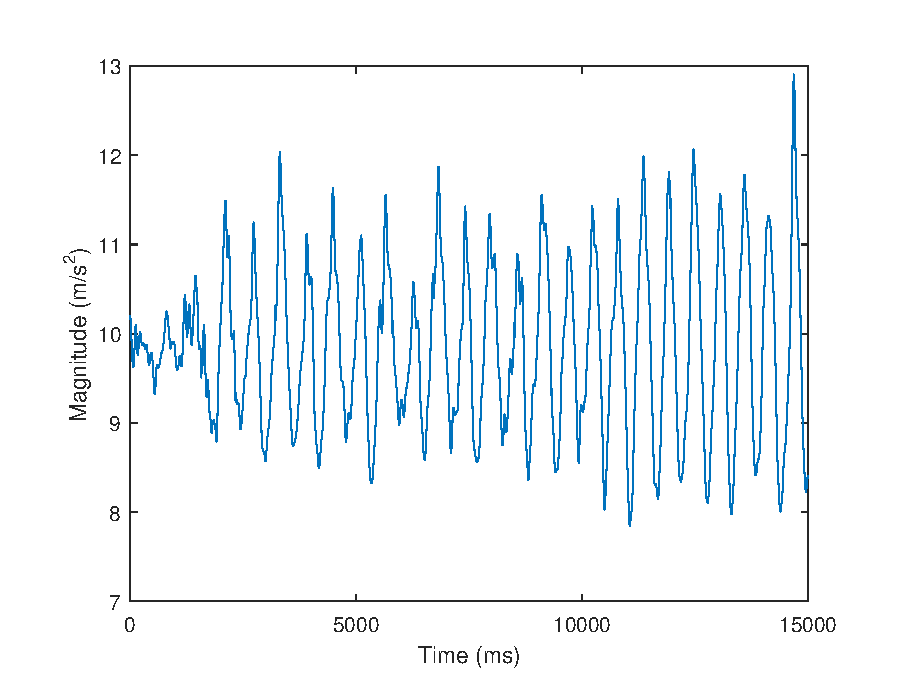
\includegraphics[width=\textwidth]{Images/accel_signal.eps}
                    \centering
                    \caption{Example of an accelerometer signal recorded during a period of walking.}
                    \label{img_accel_ex}
                \end{figure}

            \subsection{Previous Attempts}

                There have been a number of attempts to develop step counting algorithms with only an accelerometer signal.

                In Navqi, et. al. \cite{navqi} a relationship between walking speed and the magnitude of the accelerometer signal is derived and used in devising an algorithm that is based on thresholding the magnitude of the signal. The algorithm is then tested on 5 samples ranging from 16 to 44 steps and achieves an average accuracy of 96.6\%. The collection protocol is not noted besides the fact that the signal is collected by a device fixed at the centre of mass of the subject.

                In Palshikar \cite{palshikar}, the author describes a methodology of peak detection in time-series. The author describes the general flow of the method in which each point in the series is scored on how peaky it is. A search for local peaks using the standard deviation and mean of the signal is then performed. This methodology forms the basis for part of the step counting algorithm described later.

                In Brajdic and Harde \cite{brajdic}, the authors test a multitude of types of algorithms for both walk detection and step counting. The focus of this project is step counting, so walk detection algorithms will be ignored. The authors note that many algorithms involve thresholding a property of the signal, especially when the sensor is placed on the foot. However, it is mentioned that choosing an optimal threshold is difficult for different users, surfaces, or shoes. Other algorithms use peak detection or zero crossings to count steps. In the frequency domain, some algorithms look for high magnitudes of frequencies related to walking speeds to search for periods of walking and can hence calculate fractional steps. Fractional steps are defined as the dominant perceived walking frequency multiplied by the length of this period. This is done either via the Short Term Fourier Transform or Wavelet Transforms. An equivalent option to these transforms is to use the autocorrelation function in the time domain. Large magnitudes indicate high periodic activity at the lags for which they occur. All of these algorithms suffer from the problem that they will be triggered by any movement with a similar periodicity to walking. A more complex algorithm involves non-linear template matching with dynamic time warping. A generic template can be generated offline and then correlated in real time with the signal. 

                Brajdic and Harde \cite{brajdic} also explored machine learning based techniques, with commonly used features such as mean, variance, energy, entropy, correlation between axes, and Fast Fourier Transform (FFT) coefficients. They note previous attempts used classifiers such as neural networks, Gaussian mixture models, or support vector machines.

                From this list of techniques, Brajdic and Harde \cite{brajdic} chose 9 to evaluate. These 9 were: windowed peak detection, mean crossing counts, normalized autocorrleation, dynamic time warping, short term fourier transform, continuous wavelet transform, discrete wavelet transform, hidden markov model, and k-means clustering. 

                In order to evaluate all of these algorithms, the authors collected 130 data recordings from 27 subjects with a Galaxy Nexus GT-I9250 across a variety of scenarios: in hand, in a pocket, in a back pocket, or in a handbag. A video recording was taken of each session for later validation.

                With the data recordings and these algorithms, the authors concluded that the windowed peak detection and the continuous wavelet transform methods worked the best. With a median error of 1.3\% for each. Note that this was achieved with 80 of the 130 data recordings that had 'reliable ground truth step counts'. The authors also note that the placement of the phone had little effect on the step counting performance. 


        \section{Sleep Detection}

            The literature on sleep detection with a wrist-mounted accelerometer is much sparser as wearable devices are a relatively new invention. 

            In Borazio, et. al. \cite{borazio} the authors built a custom device to be worn on the wrist with an accelerometer that samples at 100Hz. They collected a dataset containing 409 hours of sleep lab data, with each data recording comprising a night's sleep from one patient. The patient underwent polysomnography to provide a ground truth. The authors proposed a simple algorithm that thresholds the acceleration signal based on the standard deviation of the magnitude. If the last 100 points (1 second of recording) exceeds a threshold, then the user is marked as not sleeping. The authors compared their method against the well known Oakley \cite{oakley} and Cole \cite{cole} algorithms that use activity counts to determine wakefulness, as well as against the ground-truth polysomnography. 

            The results show that the novel approach marginally outperforms the Oakley and Cole algorithms (79.83\% vs 74.94\% and 73.75\% respectively). The authors note that not surprisingly all the algorithms fail when the patient is awake but not moving. The dataset collected has been made publicly available and will be used to test algorithms developed in this project.

            In van Hees, et. al. \cite{vanhees}, the authors attempt to classify sleep using the arm-angle of the patient. The authors state that sleep is characterized by a period of low frequency of changes in arm-angle. The methodology consists of calculating the arm angle using rolling medians of the x, y, and z components of acceleration and then assessing changes in arm angle between 5 second epochs. If there was no change larger than $5^{\circ}$ in 5 minutes, then these were classified as sustained inactivity. The accelerometer data was collected along with a self reported sleep log of onset and offset. The authors report that overall there was moderate agreement between the results of the analysis of accelerometer data and self-reported sleep duration.